\newcommand{\ov7670_capture}{\texttt{ov7670\_capture}}

\chapter{Design and Implementation}

\section{OV7670 sensor controller}
\subsection{Overview}
To prove that the interface was suitable for image sensors a 640 x 480 OV7670 CMOS sensor was used to capture real-time image data... The Omnivision OV7670 is a small, low-cost CMOS sensor originally design for use in mobile phones which has seen popularity in the hobbyist electronics community due to its availability and ease of use. These factors, along with the wealth of documentation available contributed to its inclusion in this proof-of-concept system. Originally designed for use in resource-constrained mobile phones which lacked the power to do image processing themselves, the OV7670 contains built-in hardware for image enhancements such as de-bayering, lens correction and noise removal, making it surprisingly complex. The OV7670 was included solely to demonstrate the effectiveness of the interface in a real camera system, thus these features are not used.

\begin{figure}
  \centering
  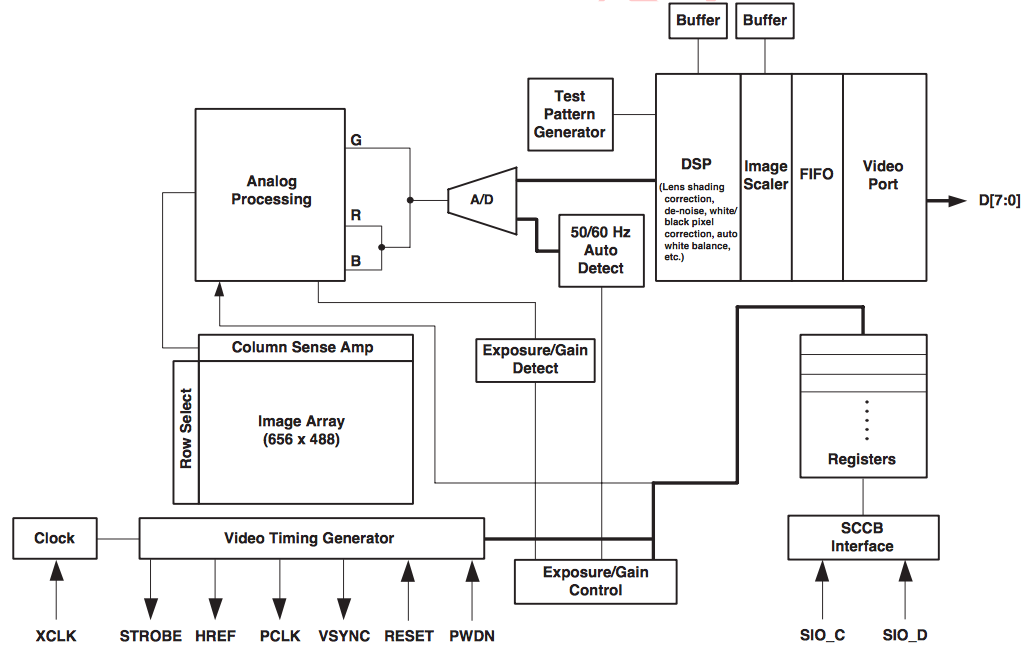
\includegraphics[width=1\textwidth]{./img/ov7670_block_diagram.png}\par
Source: Omnivision OV7670/OV7171 1.0 Specification
  \caption{Functional block diagram of Omnivision's OV7670 CMOS image sensor.}
  \label{fig:ov7670_block_diagram}
\end{figure}

Figure \ref{fig:ov7670_block_diagram} outlines the key functional blocks inside the OV7670. Light is captured by a 656 x 488 array over a specific duration of exposure. From here it is read out one row at a time into the analogue processing block which performs white-balance adjustments and amplifies the signal to increase sensitivity. From here it is digitised and fed into an image processing block for lens correction, de-noising and various other enhancements. Image scaling is also performed, before it is piped into a \gls{fifo} buffer ready for output on the 8-bit parallel video interface. The pixel size depends on the pixel format used: the RAW format only uses 8 bits and a single pixel can be output each clock cycle, while the RGB 4:2:2 and YUV 4:2:2 formats require 16 bits, thus taking two clock cycles per pixel. To construct a complete frame from the output pixels we require some additional information provided by the video timing generator in the form of vertical and horizontal synchronisation signals. The synchronisation signals in Figure \ref{fig:ov7670_timing} can be used to keep track of which the starting point of the each frame, and signals whether or not the pixel data on \texttt{D} can be sampled. 

\begin{figure}
  \centering
  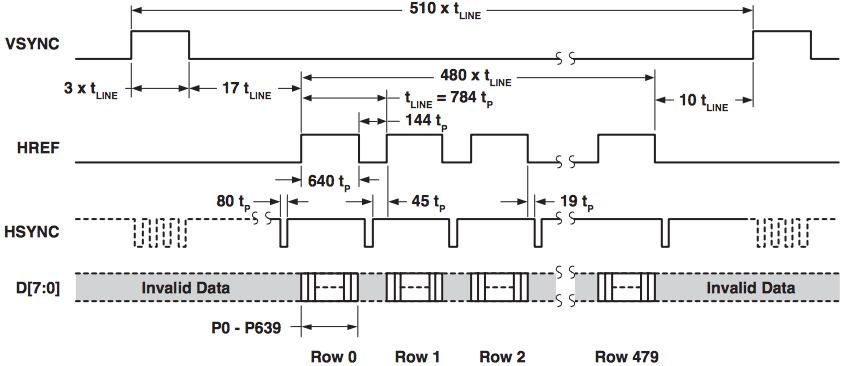
\includegraphics[width=1\textwidth]{./img/ov7670_timing.png}\par
Source: Omnivision OV7670/OV7171 1.0 Specification
  \caption{OV7670 timing diagram. The \texttt{VSYNC} signal pulses shortly before the start of each frame. \texttt{HREF} is high to indicate the data on output \texttt{D} is valid.}
  \label{fig:ov7670_timing}
\end{figure}

\subsection{\texttt{ov7670\_controller} module}
The OV7670 contains a set of internal registers to configure all aspects of its operation. In order to set the output format to 640 x 480 RAW the correct registers must be set using the \gls{sccb} protocol --- a direct clone of I\textsuperscript{2}C, renamed for licensing / IP reasons. As we are only interested in writing to specific registers there is no need to implement bidirectional I\textsuperscript{2}C communication. To drive the \gls{sccb} interface the \texttt{ov7670\_controller} module utilises I\textsuperscript{2}C code written by Mike Fields (http://hamsterworks.co.nz/mediawiki/index.php/Zedboard_OV7670). Table \ref{table:ov7670_register_settings} lists the register settings used to configure the OV7670 for 640 x 480 RAW output at 30 \gls{fps}. On powerup, the \texttt{ov7670\_controller} module performs the following actions for each register it configures:

\begin{enumerate}
    \item Pull \texttt{SDA} low to signal master is about to send
    \item Send 8-bit address frame with value 0x42
        \begin{itemize}
            \item \texttt{Bits 7--1}: OV7670 I\textsuperscript{2}C slave address \texttt{0x21}
            \item \texttt{Bit 0}    : \texttt{R/W = 0} to write to register) 
        \end{itemize}
    \item Pause to allow OV7670 to acknowledge address frame
    \item Send 8-bit data frame with address of configuration register
    \item Pause to allow OV7670 to acknowledge data frame
    \item Send a second data frame with value to write to configuration register
    \item Pause to allow OV7670 to acknowledge data frame
\end{enumerate}

The \texttt{ov7670\_controller} module contains a 'dumb' I\textsuperscript{2}C controller --- it ignores all responses from the slave and stops as soon as it has finished configuring the OV7670 registers. For the sake of simplicity, the register configuration can be re-triggered by asserting the reset signal. Not implementing intelligence to deal with frame retransmits due to errors simplifies the design significantly, while still allowing the user to manually re-trigger register configuration if anything does go wrong. Once the configuration has been written the \texttt{ov7670\_controller} module asserts the \texttt{start\_capture} signal to notify the \texttt{ov7670\_capture} module that the OV7670 is initialised and properly configured.

\begin{table}
    \begin{tabular}{llll}
    Register            & Address   & Value     & Description                       \\
    COM7                & 0x12      & 0x80      & Reset all registers to defaults   \\
    CLKRC               & 0x11      & 0x01      & Input clock prescaler divide-by-four, disable PCLK doubling (PCLK will be \(f_internal / 2\)) \\
    DBLV                & 0x6B      & 0x7A      & Input clock PLL x4                \\
    COM7                & 0x12      & 0x01      & Output format 640 x 480 Bayer RAW \\
    COM3                & 0x0C      & 0x00      & Disable output scaling            \\
    COM14               & 0x3E      & 0x00      & No PCLK scaling                   \\
    SCALING_XSC         & 0x70      & 0x3A      & Magical horizontal scale factor   \\
    SCAKING_YSC         & 0x71      & 0x35      & Magical vertical scale factor     \\
    SCALING_DCWCTR      & 0x72      & 0x11      & Downsample by 2           \\
    SCALING_PCLK_DIV    & 0x73      & 0xF0      & No PCLK scaling           \\
    SCALING_PCLK_DELAY  & 0xA2      & 0x02      & Scaling output delay 2    \\
    \end{tabular}
    \caption{(Based on values in OV7670 datasheet and implementation guide)}
    \label{table:ov7670_register_settings}
\end{table}

\subsection{\texttt{ov7670\_capture} module}
Given that the purpose of a standardised image sensor interface is to provide video data in a format which can be paired with any image sensor device, it stands to reason that the data must be converted to a different format at some point. The task of the \ov7670_capture module is to capture pixels from the OV7670's parallel video interface and pass them on to the \texttt{i\_buf\_controller} module detailed in Section \ref{sec:framebuffer_dma} for storage in the framebuffer where they are processed by the DVI encoder.

Originally the \ov7670_capture module had direct control over the memory, however this functionality was moved to the \texttt{i\_buf\_controller} module. The OV7670's video interface has very similar synchronisation signals to those required by the \texttt{i\_buf\_controller} module. 

As the video interface is used repeatedly in the proof-of-concept design it is important to understand what it is and how it works. Firstly, the term 'video interface' is used here to denote a particular set of signals with well-defined functions. 

\marginpar{NEEDS A PICTURE OF OV7670 MODULE!}

\section{Framebuffer DMA processor}
\label{sec:framebuffer_dma}

\section{DVI encoder}

Include formula for exact throughput

\section{DVI decoder}
\section{EDID subsystem}
\section{Exposure sync subsystem}
\section{Flash storage manager}
\section{Viewscreen controller}
\section{Test pattern generator}
\section{Sequence detector}